This section provides an overview of the data that has been utilized in training of models - and data that pretrained models have been trained on.

\subsection{Danish Real Estate 2019 Data (DRE19)}\label{sec:DRE19}
This dataset was collected and catalogued by the author using web crawlers targeting various danish real estate websites. 
Every one of the collected ~21.000 images are hashed and linked to a database entry, allowing for backtracking of images to an actual sales posting.
\newline
On average an apartment/house has ~21 unique images - on average ~5 of these are maps, aerial, outdoor, public facilities and non-related images.
Of the images that are of the property, apartment or house some are difficult to put into one single category or are simply not representative images.
Therefore, in order to simplify the labeling task, a significant portion of the images were disregarded.
\newline
Describing formally which images are acceptable, and which are not, is difficult due to many one-offs and outliers.
\begin{figure}[H]
    \centering
    \begin{subfigure}[b]{0.4\textwidth}
      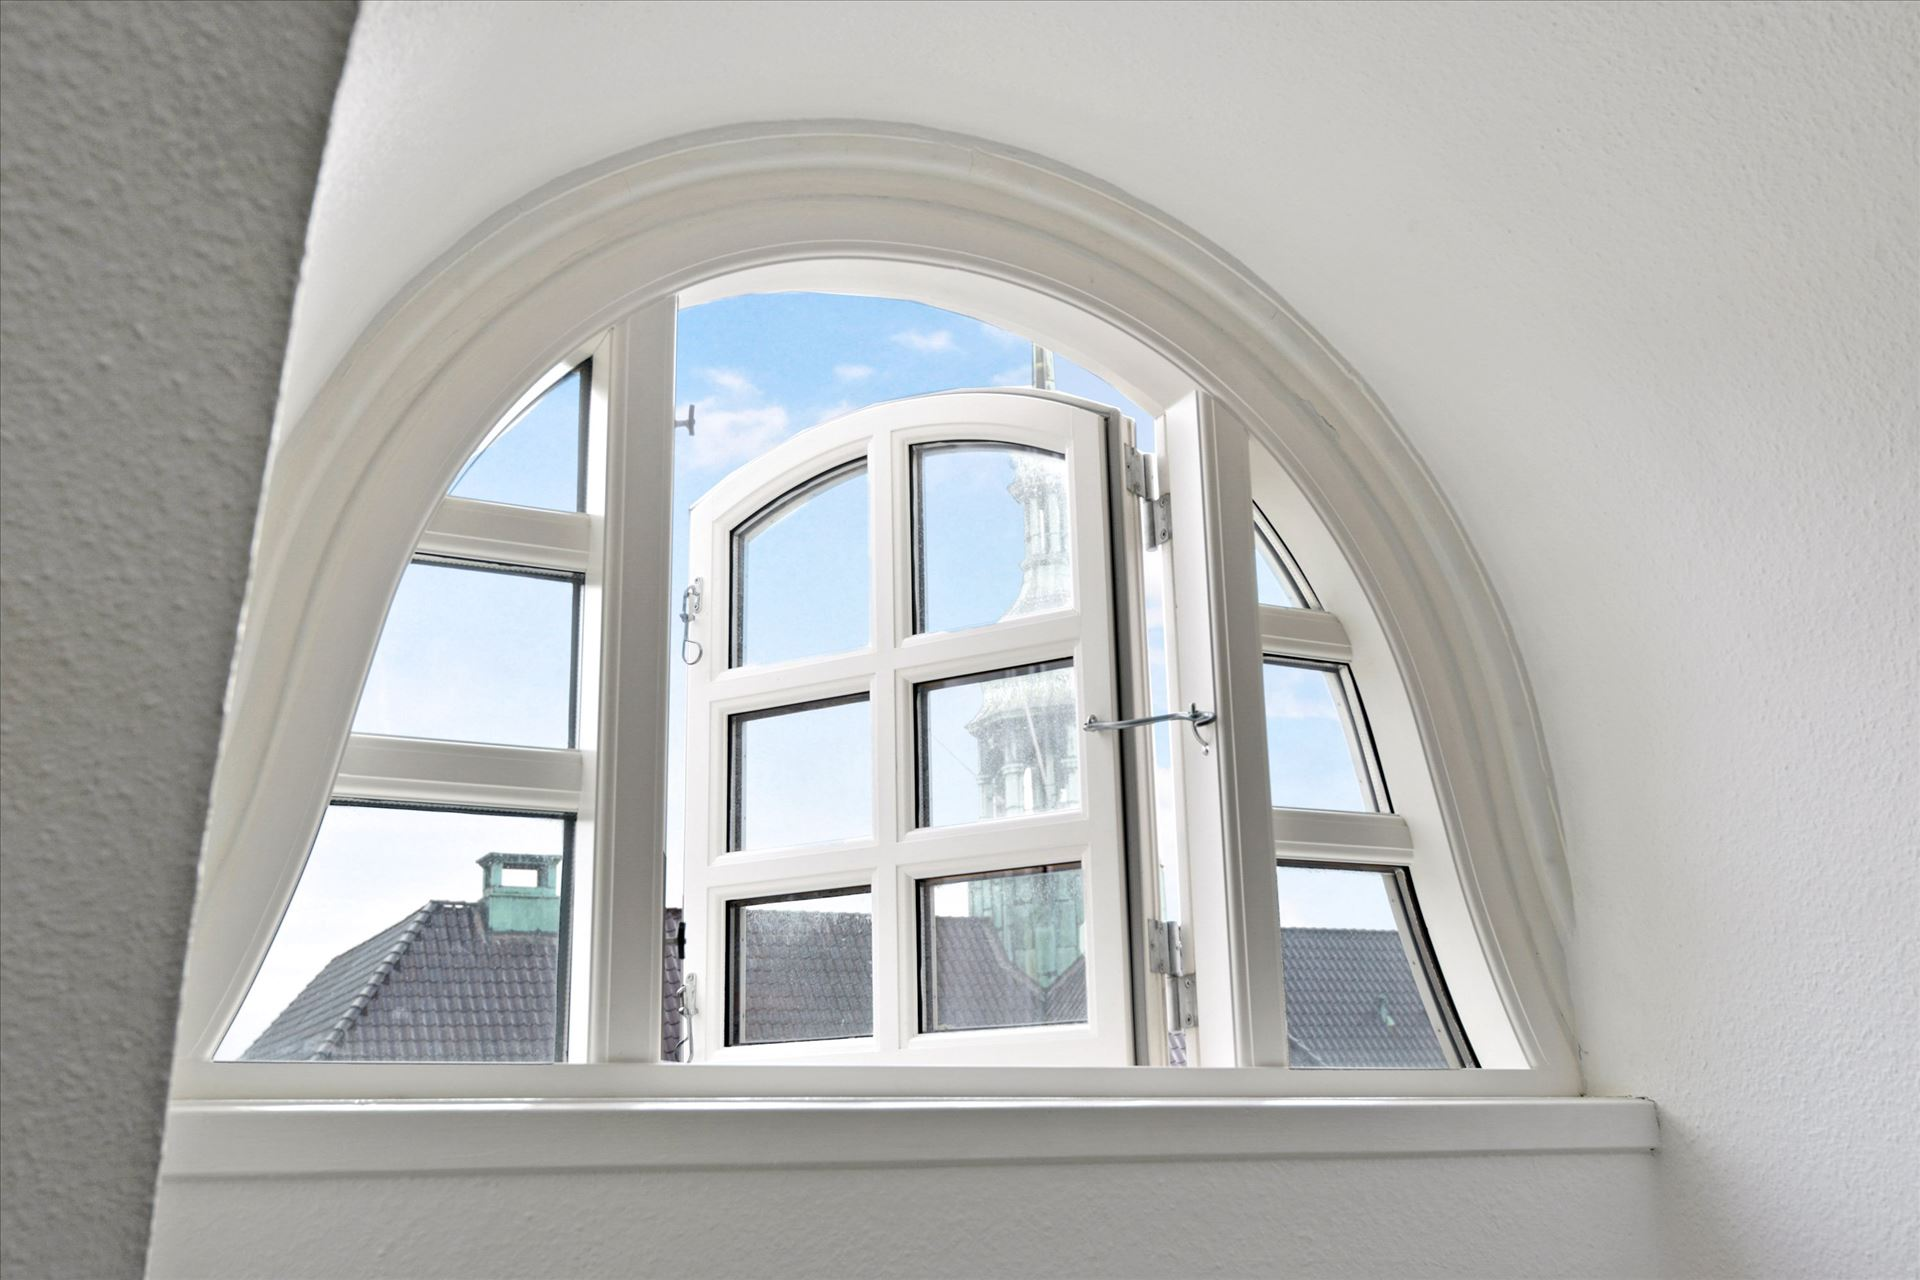
\includegraphics[width=\textwidth]{pictures/random/awindow}
      \caption{A particular object in focus}
      \label{fig:1}
    \end{subfigure}
    %
    \begin{subfigure}[b]{0.4\textwidth}
      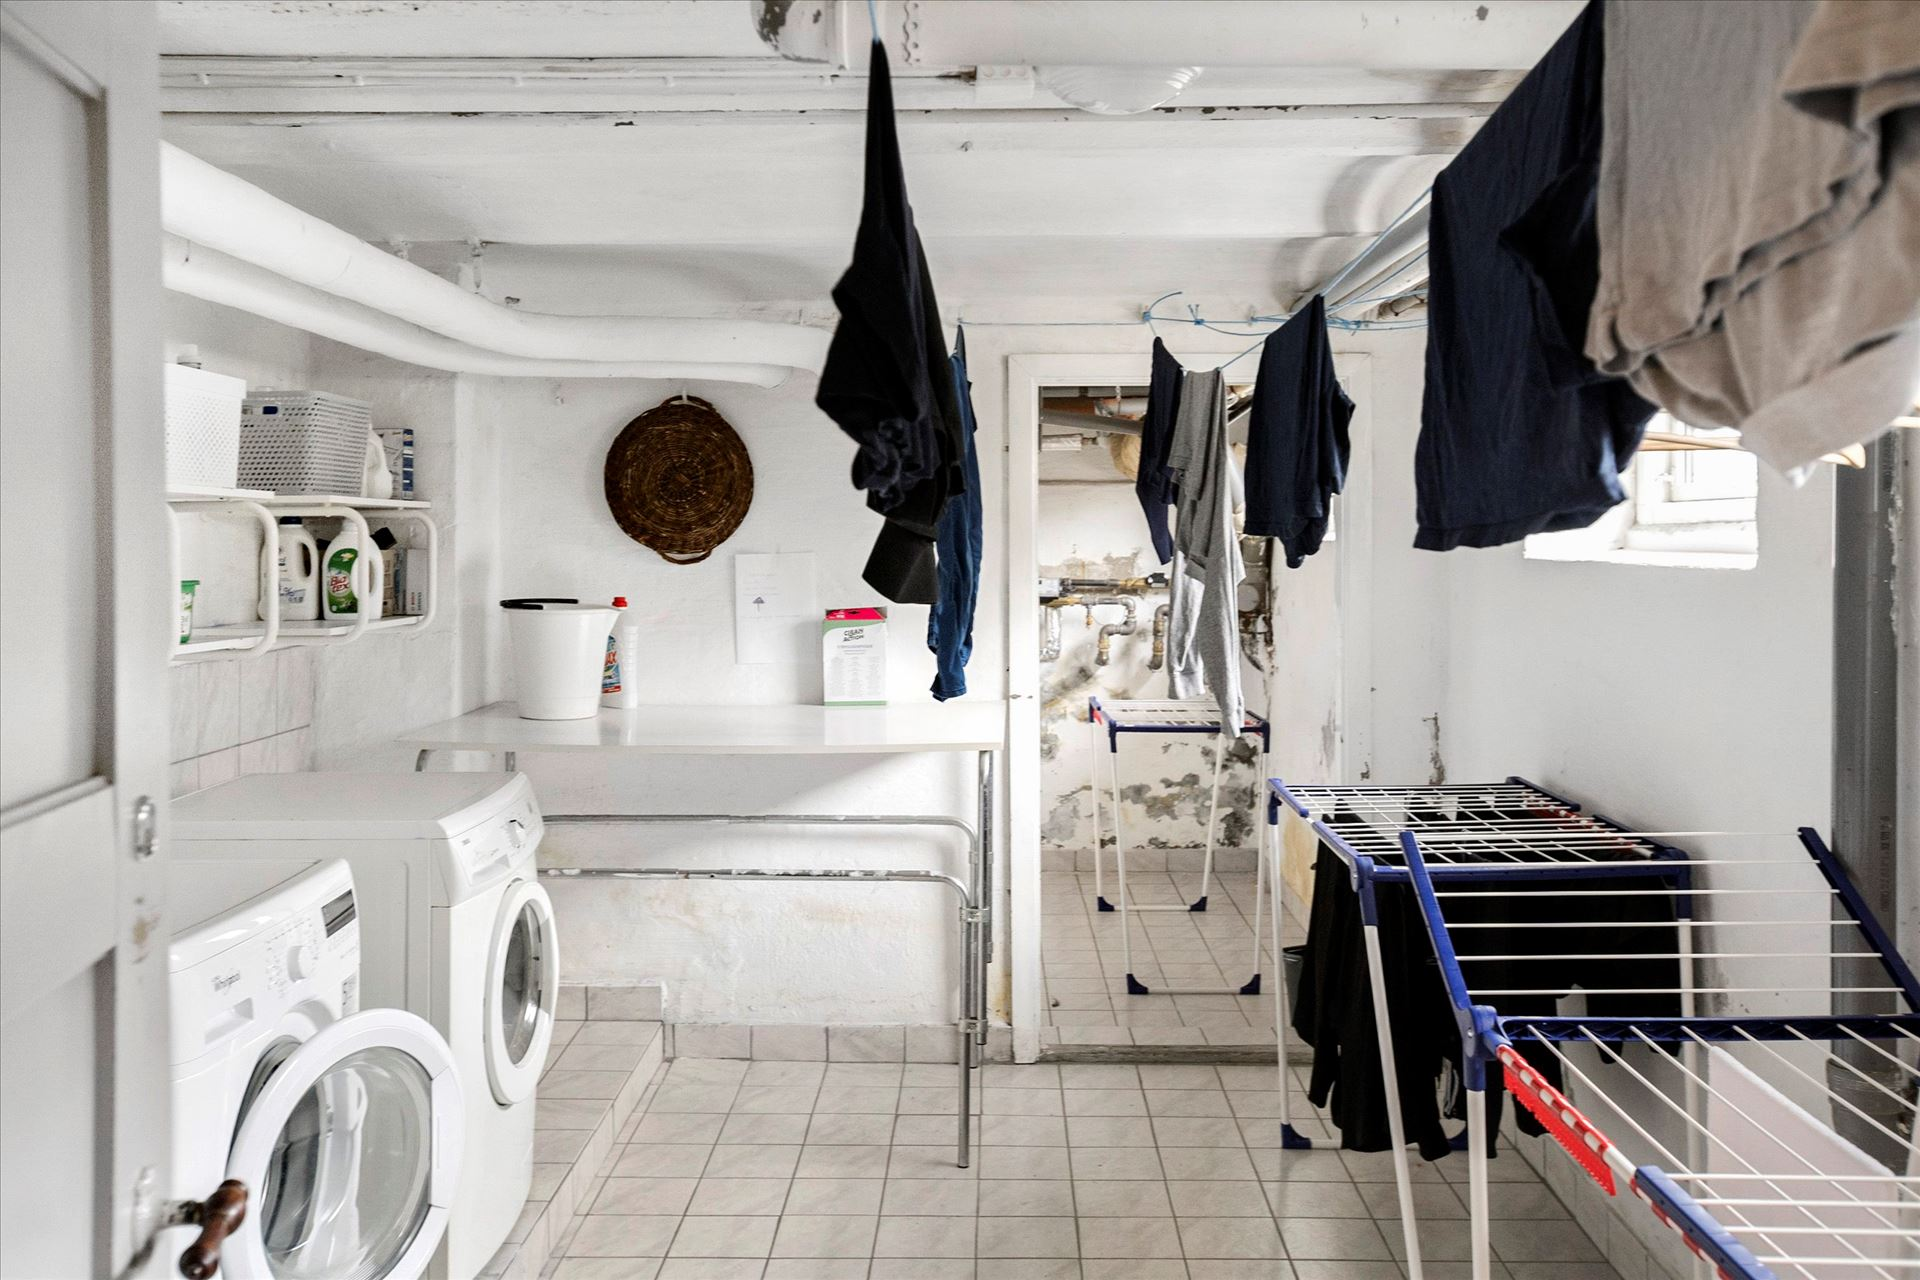
\includegraphics[width=\textwidth]{pictures/random/basement}
      \caption{Sparsely populated class; basement}
      \label{fig:2}
    \end{subfigure}
    %
    \begin{subfigure}[b]{0.4\textwidth}
      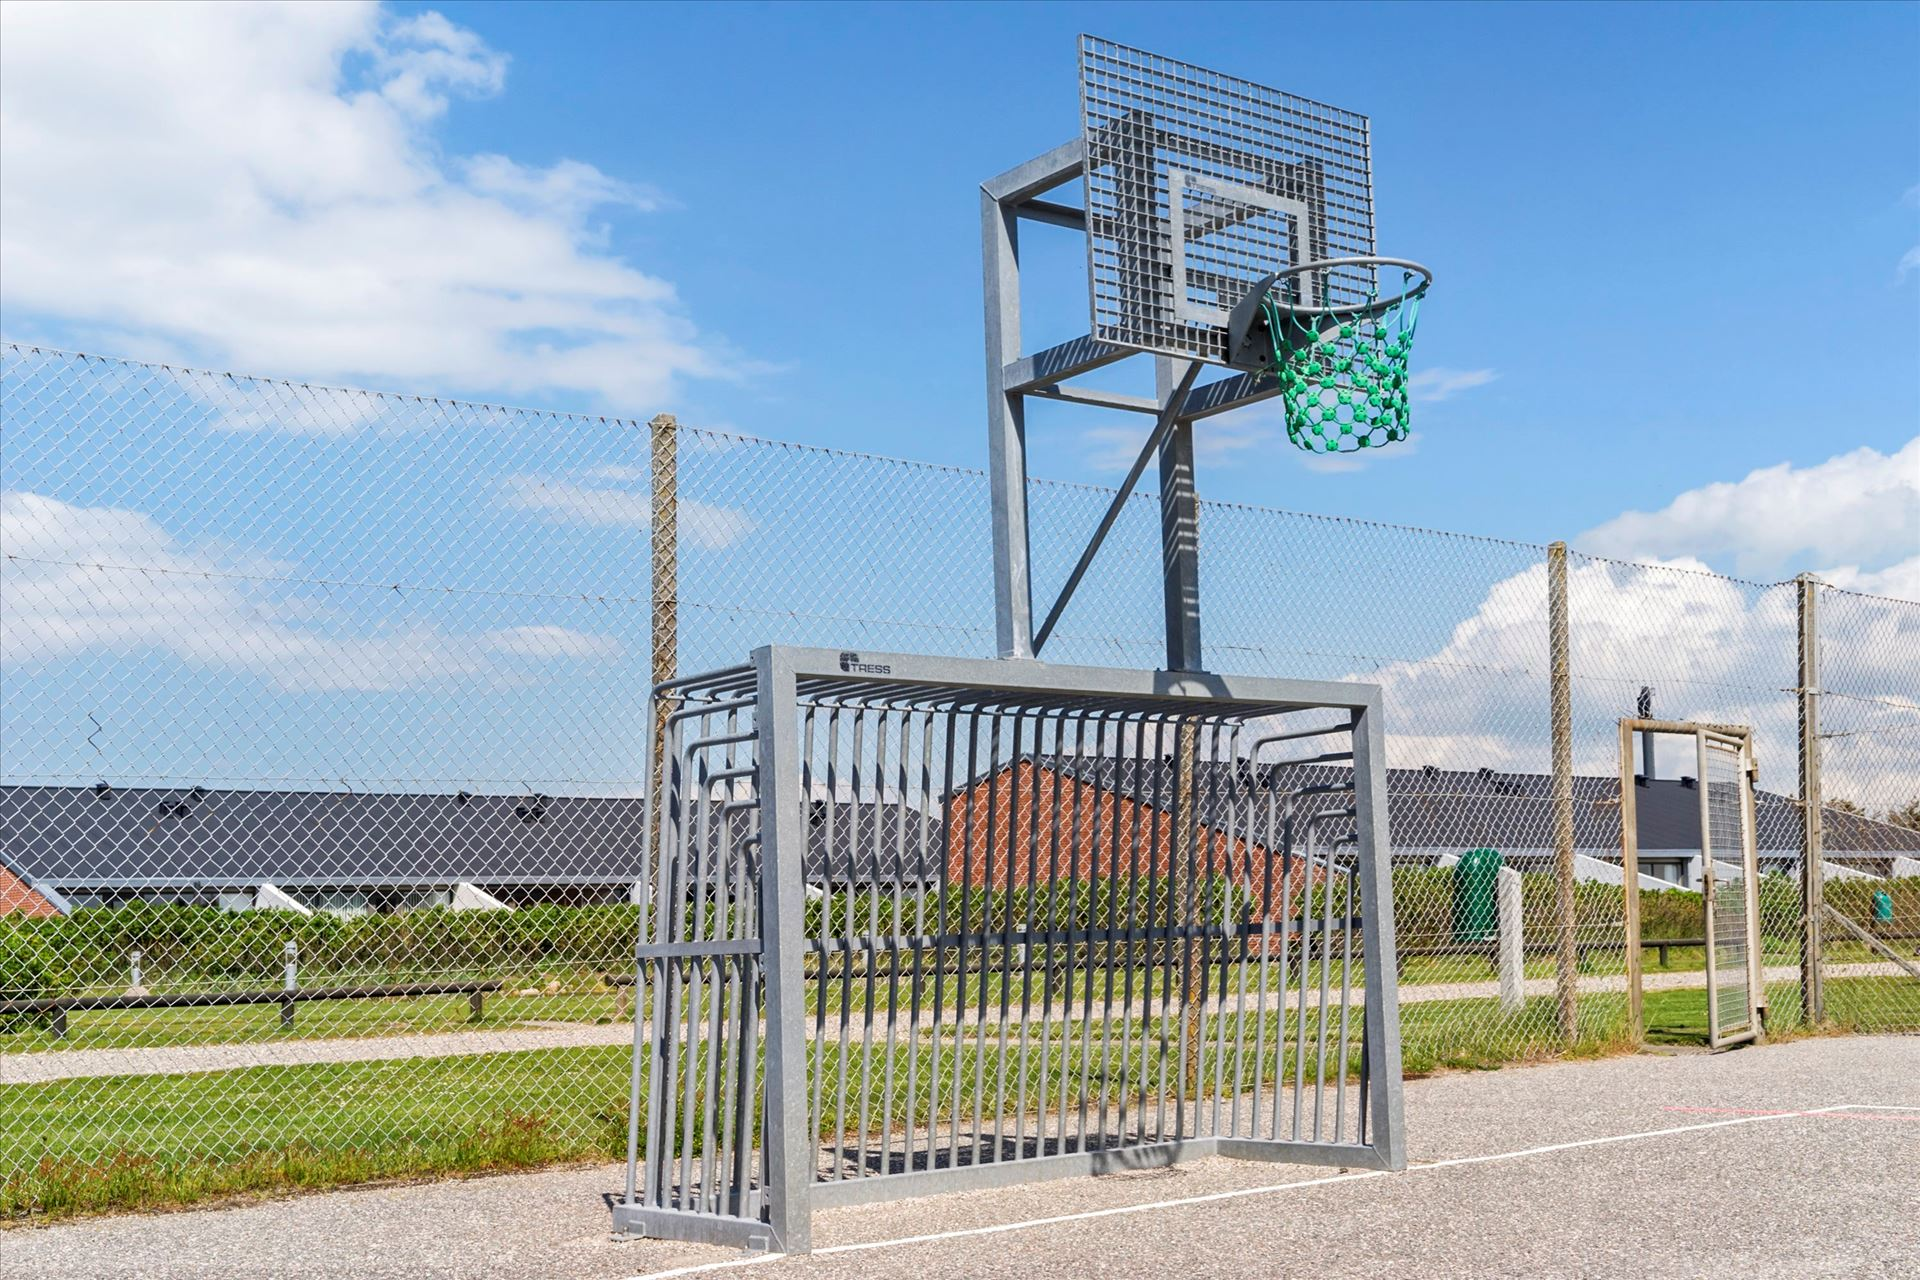
\includegraphics[width=\textwidth]{pictures/random/public}
      \caption{Unrelated to aesthetic of home}
      \label{fig:3}
    \end{subfigure}
    % 
    \begin{subfigure}[b]{0.4\textwidth}
      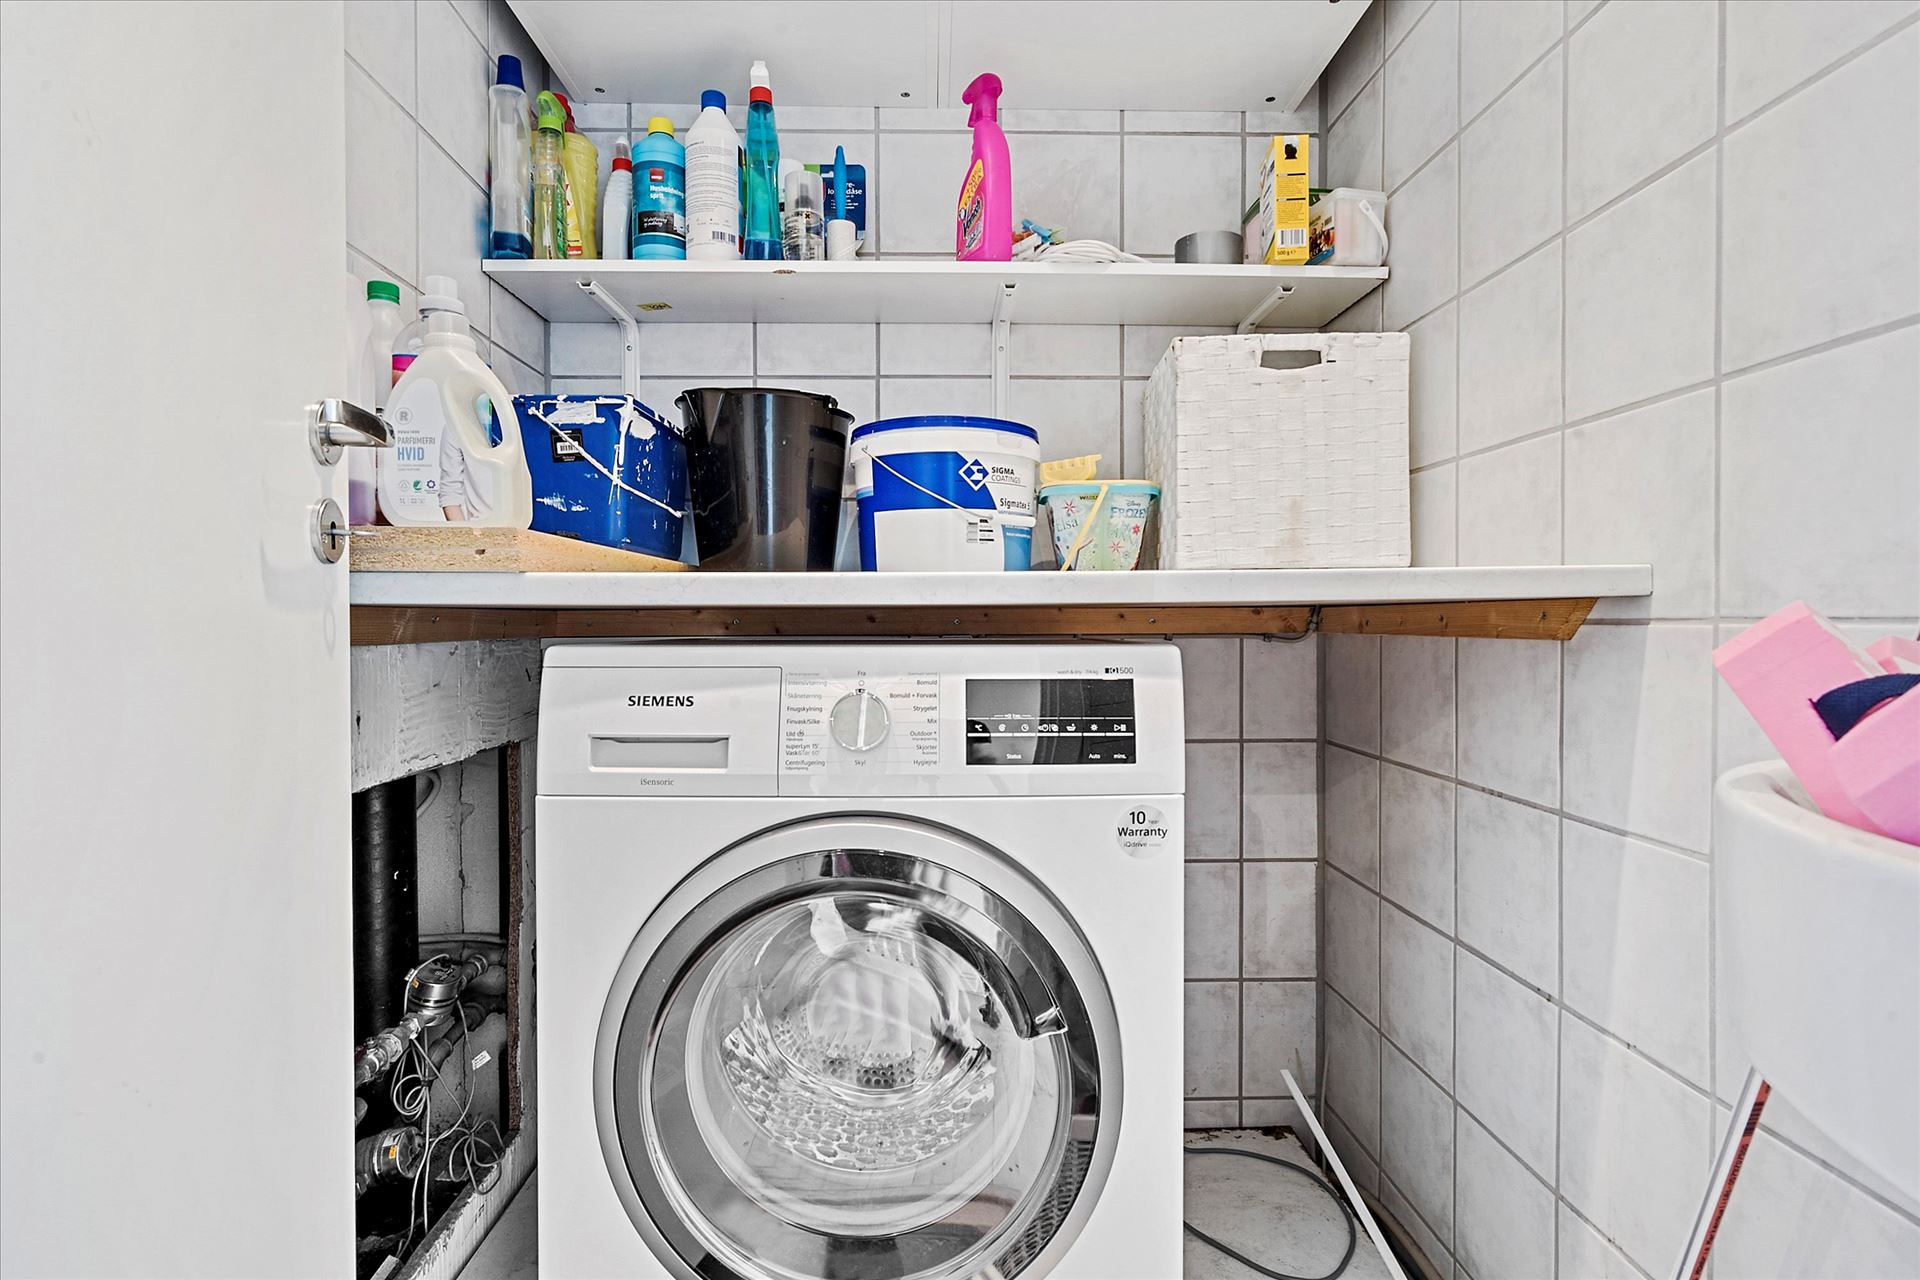
\includegraphics[width=\textwidth]{pictures/random/washer}
      \caption{Ambiguous class}
      \label{fig:4}
    \end{subfigure}
    \caption{Examples of irregular images that have been excluded}
    \label{fig:misfoster}
\end{figure}

Examples of images that have been discarded are presented in \autoref{fig:misfoster}.

Prior to labeling, data was shuffled and divided into 20 different folders, see \autoref{appendix: A}.
Ultimately 6 distinct labels were chosen to describe the images - any images that do not fall into these categories have not been considered for this project.
These labels appear to capture the majority of interior home images. In total this yielded \textbf{5458} unique, labeled images split into a 60-20-20 train-test-val split.
\begin{table}[H]
    \resizebox{\textwidth}{!}{%
    \begin{tabular}{@{}llllllll@{}}
        \toprule
        \textbf{}           & kitchen       & living\_room & bed\_room    & bath\_room   & dining\_room & entre        & \textbf{total} \\ \midrule
        \textbf{Train}      & 605           & 569          & 545          & 515          & 492          & 484          & \textbf{3310}  \\
        \textbf{Test}       & 202           & 190          & 182          & 172          & 164          & 161          & \textbf{1071}  \\
        \textbf{Validation} & 203           & 191          & 183          & 173          & 165          & 162          & \textbf{1077}  \\ \midrule
        \textbf{Total}      & \textbf{1010} & \textbf{950} & \textbf{910} & \textbf{860} & \textbf{821} & \textbf{807} & \textbf{5458}  \\ \bottomrule
        \end{tabular} %
    }
    \caption{Labeled images from various danish real-estate pages}
    \label{tab:datadist}
\end{table}